 \chapter{Przegląd SMT Solverów: Z3, Yices, cvc5}
Rozdział ten ma na celu przedstawienie SMT solverów, efektywność których zostanie zbadana w niniejszej pracy. Każdy z nich charakteryzuje się unikatową architekturą oraz zestawem funkcji, co sprawia, że są one wykorzystywane w różnych kontekstach i scenariuszach. Analiza różnic między tymi solverami pozwoli lepiej zrozumieć ich mocne strony, ograniczenia oraz potencjał w kontekście konkretnych zastosowań. W dalszej części rozdziału zostaną omówione kluczowe cechy i mechanizmy każdego z solverów, wraz z ich porównaniem pod kątem wydajności, elastyczności, oraz możliwości generowania i weryfikacji dowodów.

\section{Z3}
Z3 to wydajny SMT solver dostępny bezpłatnie przez Microsoft Research. Z3 jest solverem dla logiki symbolicznej, będącej podstawą wielu narzędzi inżynierii oprogramowania. Solvery SMT polegają na ścisłej integracji wyspecjalizowanych silników walidacyjnych. Każdy silnik jest elementem ogólnej struktury i implementuje wyspecjalizowane algorytmy. Przykładowo, silnik Z3 dla arytmetyki obejmuje Simplex, cięcia i rozumowanie wielomianowe, podczas gdy silnik dla obsługi ciągów znaków i wyrażeń regularnych korzysta z metod symbolicznych pochodnych języków regularnych. Wspólną cechą wielu algorytmów jest sposób, w~jaki wykorzystują dwoistość między znajdowaniem rozwiązań spełniających a dowodów odrzucających. Solver ten integruje również silniki do wnioskowań globalnych i lokalnych oraz globalnej propagacji.
Z3 jest używany w szerokim zakresie zastosowań inżynierii oprogramowania, obejmując weryfikację programów, walidację kompilatorów, testowanie, fuzzing przy użyciu dynamicznego wykonywania symbolicznego, rozwój oprogramowania oparty na modelach, weryfikację sieci i optymalizację.
Z3 jest programem napisanym w~C++, a zatem do jego zbudowania potrzebny jest kompilator języka C++. Zapewnia obsługę wielu języków programowania, w~tym .NET, C, C++, Java, OCaml, Web Assembly i Python.

\subsection{Architektura systemu}

Z3 integruje nowoczesny solver SAT oparty na DPLL, bazowy solver dla teorii, który obsługuje równości i funkcje nieinterpretowane, specjalistyczne silniki (dla arytmetyki, tablic itp.) oraz maszynę abstrakcyjną E-matching (dla kwantyfikatorów). Schematyczny przegląd Z3 pokazano na rysunku \ref{fig:z3}.		

\begin{figure}[htbp]
	\centering
	\begin{minipage}{\textwidth}
		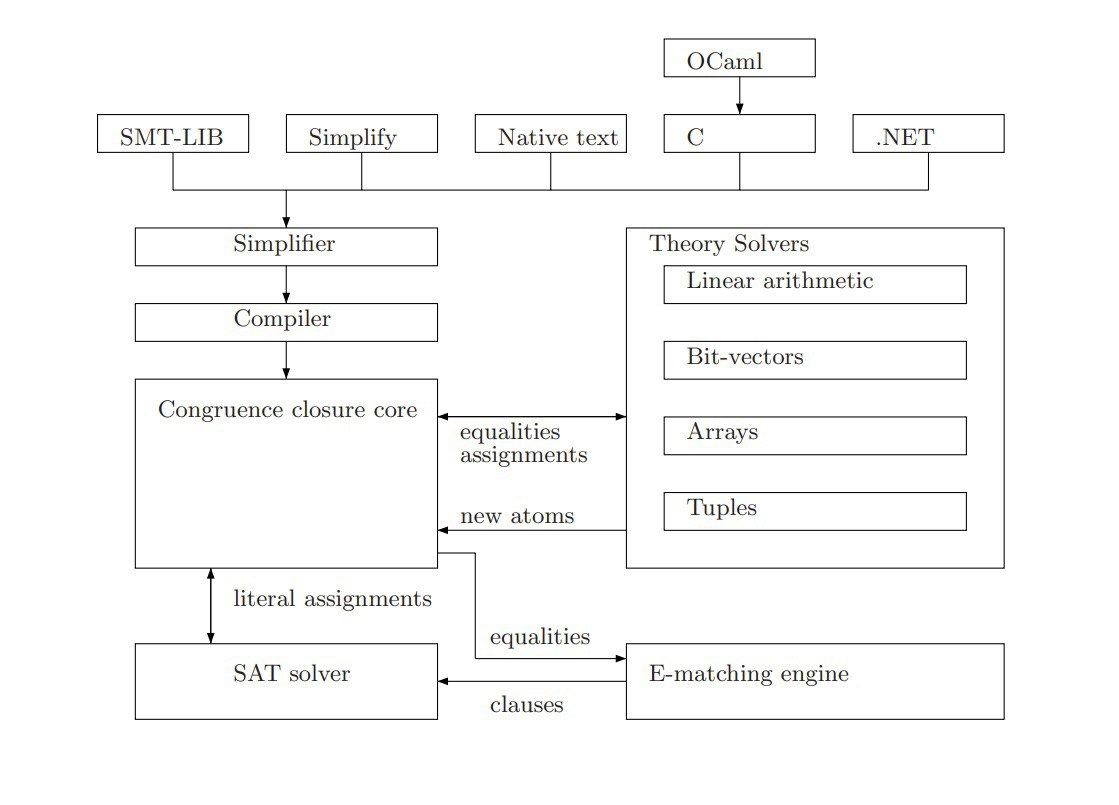
\includegraphics[width=\textwidth]{./figures/z3_architecture}
		\caption{Architektura Z3}
		\label{fig:z3}
	\end{minipage}
\end{figure}

\textbf{Simplifier}. Formuły wejściowe są najpierw przetwarzane przy użyciu niekompletnego, ale wydajnego uproszczenia. Simplifier stosuje standardowe zasady redukcji algebraicznej, takie jak $p \land true \to p$, ale także wykonuje ograniczone uproszczenie kontekstowe, identyfikując definicje równościowe w danym kontekście i redukuje pozostałą formułę przy użyciu definicji, na przykład $x = 4 \land q(x) \to x = 4 \land q(4)$. Trywialnie spełnialny spójnik $x = 4$ nie jest kompilowany do jądra, ale zachowany poza nim na wypadek, gdyby klient wymagał modelu do obliczenia $x$.

\textbf{Compiler}. Uproszczona abstrakcyjna reprezentacja drzewa składniowego formuły jest przekształcana w inną strukturę danych, składającą się ze zbioru klauzul i węzłów domknięcia kongruencji.

\textbf{Jądro domknięcia kongruencji}. Jądro domknięcia kongruencji otrzymuje przypisania prawdy do atomów od solvera SAT. Atomy obejmują równości i formuły atomowe specyficzne dla danej teorii, takie jak nierówności arytmetyczne. Równości stwierdzone przez SAT solver są przekazywane przez jądro domknięcia kongruencji za pomocą struktury danych, którą nazywamy E-grafem. Węzły w E-grafie mogą wskazywać na jeden lub więcej solverów teorii. Gdy dwa węzły są połączone, zbiór odwołań do teorii są łączone, a samo złączenie jest propagowane jako równość do solverów teorii w przecięciu obu zbiorów odwołan. Jądro również propaguje efekty solverów teorii, takie jak wywnioskowane równości oraz atomy przypisane do wartości true lub false.Solvery teorii mogą także generować nowe atomowe wyrażenia w przypadku teorii niekonweksyjnych. Te atomy są następnie integrowane i zarządzane przez główny solver SAT.

\textbf{Kombinacja teorii}. Tradycyjne metody łączenia solverów teorii opierają się na zdolności tych solverów do generowania wszystkich wynikających równości lub na wprowadzaniu dodatkowych literałów do przestrzeni poszukiwań na etapie wstępnego przetwarzania. Z3 używa nowej metody kombinacji teorii, która przyrostowo dostosowuje modele utrzymywane przez każdą teorię.

\textbf{SAT Solver}. Podziały przypadków logicznych są kontrolowane za pomocą najnowocześniejszego SAT solvera. Solver SAT integruje standardowe metody przycinania wyszukiwania, takie jak dwa obserwowane literały dla wydajnej propagacji ograniczeń boolowskich, lemma learning z wykorzystaniem klauzul konfliktowych, buforowanie faz w celu kierowania podziałami przypadków i wykonuje niechronologiczny backtracking.

\textbf{Usuwanie klauzul}. Instancjonowanie kwantyfikatorów ma skutek uboczny w postaci tworzenia nowych klauzul zawierających nowe atomy w przestrzeni poszukiwań. Z3 usuwa te klauzule wraz z ich atomami i termami, które były bezużyteczne w zamykaniu gałęzi. Klauzule konfliktowe i zawarte w nich literały nie są natomiast usuwane, dlatego instancje kwantyfikatorów, które były przydatne w wywołaniu konfliktów, są zachowywane jako efekt uboczny.

\textbf{Propagacja relewancji}. Solvery oparte na DPLL(T) przypisują wartość boolowską potencjalnie wszystkim atomom pojawiającym się w wyniku. W praktyce niektóre z tych atomów są nieistotne. Z3 ignoruje te atomy dla kosztownych teorii, jak np. wektory bitowe, i reguł wnioskowania, jak instancjonowanie kwantyfikatorów.

\textbf{Instancjonowanie kwantyfikatorów z użyciem E-matchingu}. Z3 wykorzystuje zaawansowaną technikę do rozumowania kwantyfikatorów, która opiera się na E-grafie. Dzięki nowym algorytmom, które identyfikują dopasowania w E-grafach w sposób skuteczny i przyrostowy, Z3 osiąga znaczną przewagę wydajności w porównaniu do innych nowoczesnych SMT solverów. 

\textbf{Theory Solvers}. Z3 wykorzystuje liniowy solver arytmetyczny oparty na algorytmie używanym w Yices. Teoria tablic stosuje leniwe instancjonowanie aksjomatów tablicowych. Teoria wektorów bitowych o stałym rozmiarze stosuje bitowanie do wszystkich operacji na wektorach bitowych, z wyjątkiem równości.

\textbf{Generowanie modeli}. Z3 pozwala na generowanie modeli jako części danych wyjściowych. Modele przypisują wartości do stałych na wejściu i generują częściowe grafy dla predykatów oraz symboli funkcji \cite{demoura08z}.


\section{Yices}
Yices to SMT solver, który rozwiązuje formuły zawierające niezinterpretowane symbole funkcji z równością, arytmetykę rzeczywistą i całkowitą, wektory bitowe, typy skalarne i~krotki. Yices 2 obsługuje zarówno arytmetykę liniową, jak i nieliniową.
Został opracowany w Laboratorium Informatyki SRI International przez Bruno Dutertre, Dejana Jovanovica, Stéphane Graham-Lengrand i Iana A. Masona.
Yices 2 może przetwarzać dane wejściowe zapisane w~notacji SMT-LIB (obsługiwane są zarówno wersje 2.0, jak i 1.2). Alternatywnie można pisać specyfikacje przy użyciu własnego języka specyfikacji Yices 2, który obejmuje krotki i typy skalarne. 
Yices jest oprogramowaniem open source rozpowszechnianym na licencji GPLv3. Kod źródłowy Yices jest dostępny na GitHub \cite{yices2.2}.

\subsection{Architektura systemu}
Yices 2 posiada architekturę modularną. Pozwala ona wybrać konkretną kombinację solverów teorii dla swoich potrzeb za pomocą interfejsu API lub pliku wykonywalnego yices. Dzięki API można utrzymywać kilka niezależnych kontekstów równolegle, z których każdy może wykorzystywać różne solvery i ustawienia.

Struktura oprogramowania Yices 2 jest podzielona na trzy główne moduły:

\textbf{Baza termów} Yices 2 utrzymuje globalną bazę danych, w której przechowywane są~wszystkie termy i typy.
Yices 2 zapewnia interfejs API do konstruowania termów, formuł i typów w~tej bazie danych.

\textbf{Zarządzanie kontekstem} Kontekst jest centralną strukturą danych, która przechowuje formuły twierdzeń.
Każdy kontekst zawiera zestaw twierdzeń, które mają być sprawdzane pod kątem spełnialności. Interfejs zarządzania kontekstami obsługuje operacje tworzenia i~inicjowania kontekstów, przypisywania formuł do kontekstu oraz sprawdzania ich spełnialności. Opcjonalnie kontekst może obsługiwać operacje wycofania twierdzeń przy użyciu mechanizmu push/pop. Kilka kontekstów może być konstruowanych i manipulowanych niezależnie.

Konteksty są wysoce konfigurowalne. Każdy kontekst może być skonfigurowany do obsługi określonej teorii i do korzystania z określonego solvera lub kombinacji solverów.

\textbf{Zarządzanie modelami} Jeśli zbiór formuł zadeklarowanych w kontekście jest spełnialny, to można skonstruować model formuł. Model odwzorowuje symbole formuł na konkretne wartości (np. liczby całkowite, wymierne lub stałe wektorowe). Interfejs API udostępnia funkcje do tworzenia i odpytywania modeli.

\begin{figure}[htbp]
	\centering
	\begin{minipage}{\textwidth}
		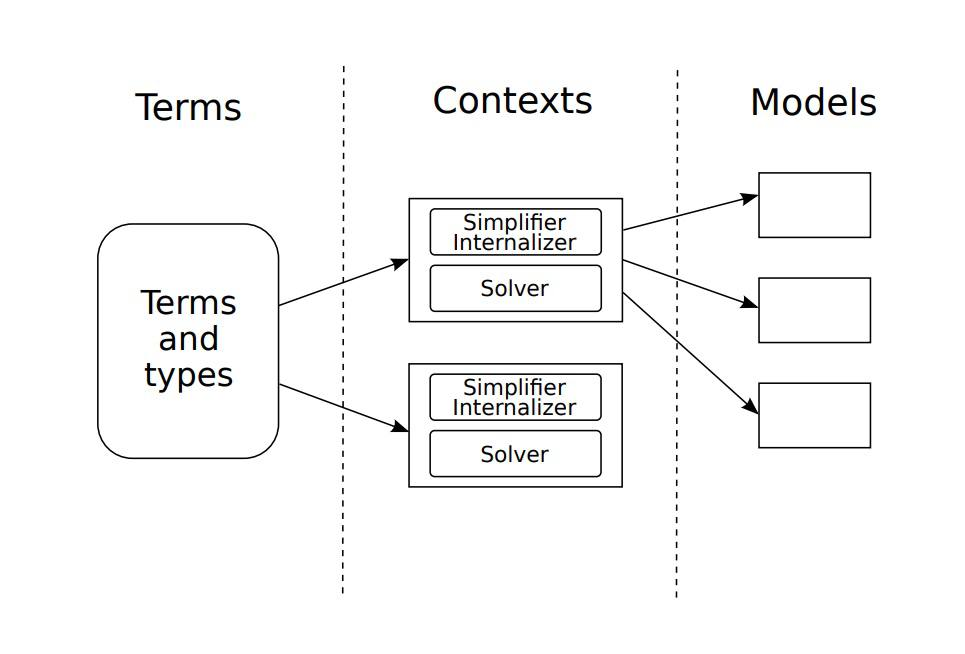
\includegraphics[width=\textwidth]{./figures/yices_architecture}
		\caption{Architektura Yices}
		\label{fig:yices}
	\end{minipage}
\end{figure}

Rysunek \ref{fig:yices} przedstawia najwyższy poziom architektury Yices 2, podzielony na trzy główne moduły. Każdy kontekst składa się z dwóch oddzielnych komponentów: Solver wykorzystuje Boolean satisfiability solver i procedury decyzyjne do określania, czy formuły zawarte w kontekście są spełnialne. Upraszczacz/internalizator konwertuje format używany przez bazę danych termów do wewnętrznego formatu używanego przez solver. W szczególności
internalizator przepisuje wszystkie formuły do koniunkcyjnej postaci normalnej, z~czego korzysta wewnętrzny SAT solver \cite{yices2.2}.


\section{cvc5}
Narzędzia z kategorii CVC (cooperating validity checker) odgrywają ważną rolę zarówno w badaniach, jak i w praktyce. Najnowsze wcielenie, CVC4, było przepisaną od podstaw wersją CVC3, napisaną w celu stworzenia elastycznej i wydajnej architektury, która mogłaby przetrwać w przyszłości. cvc5, kolejny solver z tej serii, nie jest
przepisaniem CVC4 lecz bazuje na jego sprawdzonej architekturze i bazie kodu. W porównaniu do innych solverów SMT, cvc5 zapewnia zróżnicowany zestaw teorii (wszystkie standardowe teorie SMT-LIB i wiele niestandardowych) oraz funkcjonalności poza SMT, takie jak rozumowanie wyższego rzędu i~synteza sterowana składnią (SyGuS). Zmiana nazwy raczej odzwierciedla zarówno nowy zespół programistów, jak również znaczącą ewolucję, jaką narzędzie przeszło od czasu opisania CVC4 w 2011 roku. Ponadto, cvc5 zawiera aktualizowaną dokumentację, nowe i ulepszone interfejsy API oraz bardziej przyjazną dla użytkownika instalację. Co najważniejsze, wprowadzono kilka istotnych nowych funkcji. Podobnie jak jego poprzednicy, cvc5 jest dostępny na~3-klauzulowej licencji BSD open source i działa na wszystkich głównych platformach (Linux, macOS, Windows).

cvc5 to wspólny projekt prowadzony przez Uniwersytet Stanforda i Uniwersytet Iowa \cite{BarbosaBBKLMMMN22}.

\subsection{Architektura systemu}

cvc5 obsługuje rozumowanie w zakresie formuł bezkwantyfikatorowych i kwantyfikatorowych w szerokim zakresie teorii tła, w tym wszystkich teorii standaryzowanych w SMT-LIB. Ponadto wspiera kilka niestandardowych teorii i rozszerzeń. Należą do nich, między innymi, logika separacji, teoria sekwencji, teoria zbiorów skończonych i relacji oraz rozszerzenie teorii liczb rzeczywistych o funkcje transcendentalne. 

Ogólny przegląd architektury systemu przedstawiono na rysunku \ref{fig:cvc5}.

\begin{figure}[htbp]
	\centering
	\begin{minipage}{\textwidth}
		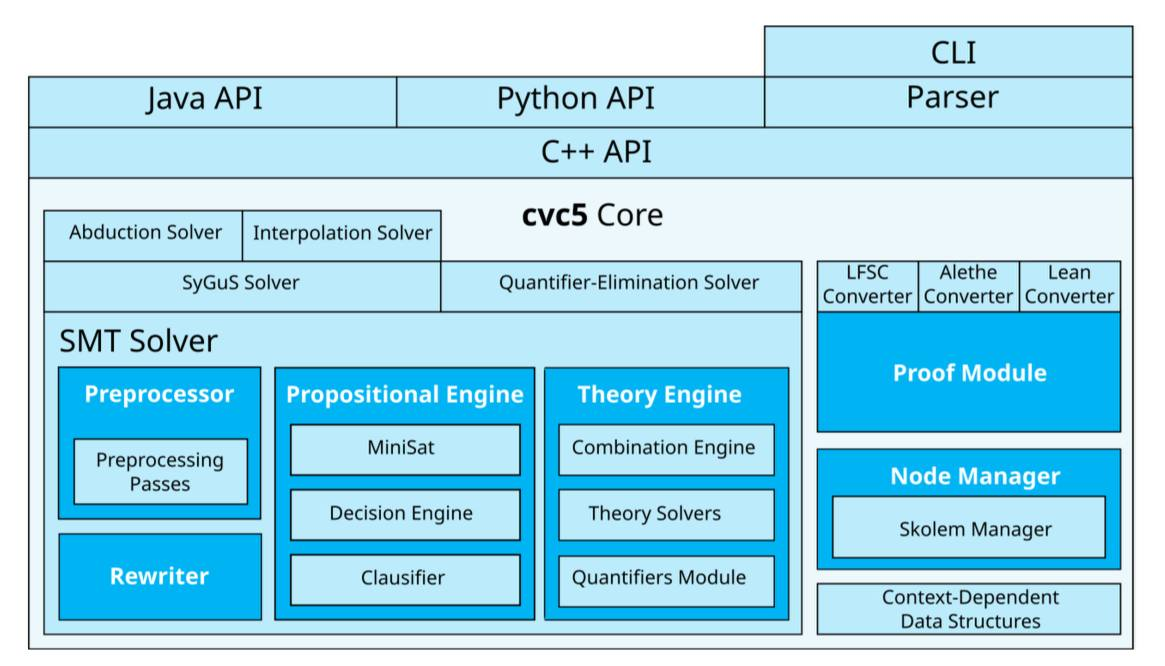
\includegraphics[width=\textwidth]{./figures/cvc5_architecture}
		\caption{Architektura cvc5}
		\label{fig:cvc5}
	\end{minipage}
\end{figure}

Centralnym elementem cvc5 jest moduł SMT Solver, oparty na frameworku CDCL(T) \cite{NieuwenhuisOT06} i dostosowanej wersji solvera propozycyjnego MiniSat. Moduł ten składa się z kilku komponentów: modułów Rewriter i Preprocessor, które stosują uproszczenia odpowiednio lokalnie (na poziomie wyrażenia) i globalnie (na całej formule wejściowej); Propositional Engine, który służy jako menedżer dla CDCL(T) SAT solvera; oraz Theory Engine, który zarządza kombinacją teorii i wszystkimi procedurami rozumowania kwantyfikatorowego.

Oprócz standardowego sprawdzania spełnialności, cvc5 zapewnia dodatkową funkcjonalność, taką jak abdukcja, interpolacja, synteza kierowana składnią (SyGuS) oraz eliminacja kwantyfikatorów. Każda z tych funkcji jest zaimplementowana jako dodatkowy solver zbudowany na bazie modułu SMT Solver. SyGuS jest głównym punktem wejścia
dla zapytań o~syntezę, które kodują problemy SyGuS jako problemy spełnialności (wyższego rzędu) z ograniczeniami semantycznymi i syntaktycznymi. Quantifer Elimination Solver wykonuje eliminację kwantyfikatorów w oparciu o śledzenie instancji kwantyfikatorów przez SMT Solver. Abduction Solver i Interpolation Solver są oparte na SyGuS, a zatem są zbudowane jako warstwy nad modułem SyGuS Solver \cite{BarbosaBBKLMMMN22}.

cvc5 zapewnia API C++ jako główny interfejs, nie tylko dla zewnętrznego oprogramowania klienta, ale także dla własnego parsera i dodatkowych wiązań języka w Javie i Pythonie. cvc5 dostarcza również tekstowy interfejs wiersza poleceń (CLI), zbudowany na parserze, który obsługuje języki wejściowe SMT-LIBv2, SyGuS2 i TPTP. Moduł Proof może wyprowadzać formalne dowody niespełnialności w trzech formatach: Lean 4 \cite{Moura021}, Alethe \cite{abs-2107-02354} i LFSC \cite{StumpORHT13}.

\subsubsection{Moduł SMT Solver} Moduł ten odpowiada za obsługę wszystkich zapytań SMT. Jego funkcjonalność obejmuje, oprócz sprawdzania spełnialności, konstruowanie modeli dla formuł spełnialnych oraz wyodrębnianie założeń, rdzeni i obiektów dowodu dla formuł niespełnialnych. Główne składniki modułu są opisane poniżej.

\textbf{Preprocessor} Przed jakąkolwiek weryfikacją spełnialności cvc5 stosuje do każdej formuły z problemu wejściowego sekwencję transformacji zachowujących spełnialność Te transformacje obejmują normalizacje, uproszczenia i przekształcenia formuł między różnymi logikami. Preprocesor wykonuje 34 różne transformacje, które mogą być dostosowywane poprzez opcje konfiguracyjne.

\textbf{Silnik Propozycyjny} Jest to podstawowy silnik CDCL(T) \cite{NieuwenhuisOT06}, który przekształca abstrakcje logiczne formuł wejściowych w postać CNF i korzysta z MiniSat jako podstawowego solvera SAT. Silnik ten używa także mechanizmów decyzyjnych do dostosowywania heurystyk wyboru decyzji.

\textbf{Przepisywacz} Ten submoduł jest odpowiedzialny za przekształcanie termów według reguł przepisywania na semantycznie równoważne postacie normalne. W przeciwieństwie do~preprocessora działa na termach w trakcie rozwiązywania problemu i jest wykorzystywany przez inne komponenty cvc5 \cite{NotzliRBNPBT19}.

\textbf{Silnik Teorii} Jest to główny składnik odpowiedzialny za sprawdzanie spójności teorii literałów, zatwierdzonych przez Silnik Propozycyjny. Koordynuje on działanie różnych solverów teorii, które obsługują różnorodne dziedziny matematyczne, takie jak arytmetyka liniowa, nieliniowa, tablice, bit-wektory, typy danych, arytmetyka zmiennoprzecinkowa, zbiory i relacje, logika separacji, stringi i sekwencje oraz funkcje niezinterpretowane.

\textbf{Solvery Teorii} cvc5 obsługuje szeroki zakres teorii, w tym arytmetykę liniową, nieliniową, tablice, bit-wektory, typy danych, arytmetykę zmiennoprzecinkową, zbiory i relacje, logikę separacji, łańcuchy znaków oraz funkcje niezinterpretowane. Ponadto wszystkie teorie przekazują kroki rozumowania do reszty systemu za pośrednictwem Menedżera wnioskowania teorii. Każdy z tych solverów emituje lematy, klauzule konfliktowe i propagowane literały za~pośrednictwem tego interfejsu \cite{BarbosaBBKLMMMN22}.

\subsubsection{Proof Module} Moduł Dowodów w cvc5 został zbudowany od podstaw, zastępując system dowodowy CVC4 \cite{HadareanBRTD15}, który był niekompletny i cierpiał z powodu licznych wad architektonicznych. Projektowanie modułu Dowodów cvc5 kierowało się kilkoma zasadami: minimalizacją narzutu czasowego generowania dowodów, zapewnieniem wystarczająco szczegółowych dowodów umożliwiających efektywne sprawdzanie, elastycznością w emitowaniu dowodów w różnych formatach oraz minimalizacją wyłączania komponentów systemu w trybie produkcji. Moduł Dowodów w cvc5 generuje szczegółowe dowody dla prawie wszystkich teorii, reguł przepisywania, przejść wstępnych, wewnętrznych solverów SAT oraz silników kombinacyjnych teorii. Dodatkowo obsługuje on produkowanie dowodów zarówno natychmiastowe, jak i leniwe, z~wbudowaną rekonstrukcją dowodów \cite{ReynoldsWBBLT17}. cvc5 jest w stanie emitować dowody w różnych formatach, w tym tych obsługiwanych przez tester dowodów LFSC \cite{StumpORHT13}, oraz asystenty dowodowe Isabelle/HOL \cite{NipkowPW02}, Lean 4 \cite{Moura021} i Coq \cite{BertotC04}.

\subsubsection{Node Manager} W cvc5 formuły i termy są reprezentowane jednolicie jako wierzchołki w grafie skierowanym acyklicznym, zarządzane przez Menedżera Węzłów. Menedżer Węzłów zarządza również Menedżerem Skolema, odpowiedzialnym za śledzenie symboli Skolema wprowadzanych podczas rozwiązywania. Węzły są niezmienne i są współdzielone za pomocą techniki hash consing, co zapewnia efektywne zarządzanie pamięcią i sprawdzanie równości składniowej w czasie stałym. Menedżer Skolema centralnie generuje stałe Skolema, co pozwala na deterministyczne generowanie nowych stałych podczas rozwiązywania i minimalizację ich liczby dla wydajności \cite{ReynoldsNBT20}. 

\subsubsection{Context-Dependent Data Structures} Aby wspierać aplikacje SMT wymagające wielokrotnych sprawdzeń spełnialności podobnych twierdzeń, cvc5 definiuje pojęcie poziomu kontekstu i wdraża kontekstowo zależne struktury danych. Te struktury zachowują się podobnie do odpowiadających im mutowalnych struktur danych w standardowej bibliotece C++, ale są związane z poziomem kontekstu i automatycznie zapisują oraz przywracają swój stan wraz ze zmianą kontekstu \cite{BarbosaBBKLMMMN22}.

\section{Analiza porównawcza SMT solverów}

Porównując Z3, Yices i cvc5, należy zwrócić uwagę na to, że każdy z tych solverów ma swoje unikalne cechy, które wpływają na sposób ich użytkowania oraz efektywność rozwiązywania problemów.

Z3 wyróżnia się wydajną architekturą opartą na wewnętrznym mechanizmie tzw. tłumaczenia zadań SMT na zadania SAT (ang. Satisfiability Modulo Theories to Boolean Satisfiability). Dzięki wsparciu dla szerokiego zakresu teorii i bogatej dokumentacji, Z3 jest często wybierany w projektach związanych z analizą i weryfikacją oprogramowania, a także w badaniach naukowych z obszaru informatyki teoretycznej i sztucznej inteligencji. Na przykład, firmy z branży technologicznej, takie jak Google i Facebook, korzystają z Z3 do weryfikacji oprogramowania oraz do analizy złożoności algorytmów.

Yices, z kolei, cechuje się prostotą użytkowania oraz wysoką efektywnością w rozwiązywaniu problemów SAT i SMT. Jego architektura koncentruje się na szybkim i niezawodnym rozwiązywaniu problemów, co czyni go popularnym wyborem w projektach związanych z~weryfikacją układów cyfrowych oraz w automatycznym generowaniu testów. Przykładowo, firmy z sektora technologii mobilnych, takie jak Samsung i Apple, wykorzystują Yices do weryfikacji poprawności działania swoich urządzeń oraz do optymalizacji procesów projektowania.

Natomiast cvc5, będący inicjatywą naukową, oferuje elastyczną i modułową architekturę, która umożliwia integrację różnorodnych technik, takich jak SyGuS oraz zaawansowane mechanizmy dowodzenia.  Jego silnik dedykowany do analizy teorii sprawia, że jest często wybierany w projektach badawczych z zakresu informatyki teoretycznej oraz w badaniach nad metodami rozwiązywania problemów SAT i SMT. Na przykład, instytucje naukowe oraz centra badawcze, takie jak MIT i Stanford University, wykorzystują cvc5 do analizy złożoności obliczeniowej algorytmów oraz do badania właściwości języków programowania.

Te różnice w architekturze i funkcjonalnościach solverów SMT mają istotne implikacje dla ich wykorzystania w praktyce. Przyjrzenie się konkretnym zastosowaniom tych solverów może dostarczyć cennych wskazówek przy wyborze odpowiedniego narzędzia.

